\documentclass[12pt,a4paper]{article}
\usepackage[utf8]{inputenc}
%加這個就可以設定字體
\usepackage{fontspec}
%使用xeCJK,其他的還有CJK或是xCJK
\usepackage{xeCJK}
\usepackage{enumerate}
%設定英文字型,不設的話就會使用預設的字型
\usepackage{hyperref}
\usepackage{graphicx}
\usepackage{geometry}
\geometry{a4paper,scale=0.8}
\setmainfont{Times New Roman}
\usepackage{listings}
\lstset{language=python}
%設定中英文的字型
%字型的設定可以使用系統內的字型,而不用像以前一樣另外安裝
\setCJKmainfont{標楷體}
%以下是新增的自定义格式更改
\usepackage[]{caption2} %新增调用的宏包
\renewcommand{\figurename}{fig} %重定义编号前缀词
%中文自動換行
\XeTeXlinebreaklocale "zh"

%文字的彈性間距
\XeTeXlinebreakskip = 0pt plus 1pt

%設定段落之間的距離
\setlength{\parskip}{0.3cm}
\title{}
\author{虎尾科技大學\\40723115\\ 林于哲}
\date{April 1 2021}
\renewcommand{\contentsname}{目錄} %將content轉為目錄
\begin{document}
\maketitle
\tableofcontents

%摘要開始部分
\newpage
\begin{huge}\textbf{Introduction}\end{huge}\\
\begin{itemize}
\item Activation Function 
   \begin{enumerate}[I.]
   \item Sigmoid Function
   \item Relu
   \end{enumerate}
\end{itemize}   
\begin{itemize}
\item Optimizer
   \begin{enumerate}[I.]
   \item Adam
   \item SigmoidPrime
   \end{enumerate}
\end{itemize}  
\begin{itemize}   
\item Loss function
   \begin{enumerate}[I.]
   \item Mean Squared Error
   \end{enumerate}
\end{itemize} 
\section{為何 deep learning 會在此時崛起?}
Four major trends in scientific computing have become increasingly important for deep learning.\\

(1) 支援張量運算程式語言與程式庫的崛起 First, starting in the 1960s, the development of domain specific languages such as APL, MATLAB, R and Julia, turned multidimensional arrays (often referred to as tensors) into first-class objects supported by a comprehensive set of mathematical primitives (or operators) to manipulate them.\\
Separately, libraries such as NumPy, Torch, Eigen and Lush made array-based programming productive in general purpose languages such as Python, Lisp, C++ and Lua.\\

(2) 自動求導數套件的開發 Second, the development of automatic differentiation made it possible to fully automate the daunting labor of computing derivatives. This made it significantly easier to experiment with different machine learning approaches while still allowing for efficient gradient based optimization. The autograd package popularized the use of this technique for NumPy arrays, and similar approaches are used in frameworks such as Chainer, DyNet, Lush, Torch, Jax and Flux.jl.\\

(3) 自由開源軟體的普及 Third, with the advent of the free software movement, the scientific community moved away from closed proprietary software such as Matlab, and towards the open-source Python ecosystem with packages like NumPy, SciPy, and Pandas. This fulfilled most of the numerical analysis needs of researchers while allowing them to take advantage of a vast repository of librariesto handle dataset preprocessing, statistical analysis, plotting, and more.\\
Moreover, the openness, interoperability, and flexibility of free software fostered the development of vibrant communities that could quickly address new or changing needs by extending the existing functionality of a library or if needed by developing and releasing brand new ones. While there is a rich offering of open-source software for neural networks in languages other than Python, starting with Lush in Lisp, Torch in C++, Objective-C and Lua, EBLearn in C++, Caffe in C++, the network effects of a large ecosystem such as Python made it an essential skill to jumpstart one’s research. Hence, since 2014,most deep learning frameworks converged on a Python interface as an essential feature.\\

(4) 多核 GPU 運算的發展 Finally, the availability and commoditization of general-purpose massively parallel hardware such as GPUs provided the computing power required by deep learning methods. Specialized librariessuch as cuDNN, along with a body of academic work (such as Andrew Lavin. maxdnn: An efficient convolution kernel for deep learning with maxwell gpus,January 2015 and Andrew Lavin and Scott Gray. Fast algorithms for convolutional neural networks.2016 IEEEConference on Computer Vision and Pattern Recognition (CVPR), pages 4013–4021, 2016), produced aset of high-performance reusable deep learning kernels that enabled frameworks such as Caffe,Torch7, or TensorFlow to take advantage of these hardware accelerators.\\

\section{What is Reinforcement Learning?}
強化學習是通過agent與已知或未知的環境持互動,不斷適應與學習,得到的回饋可能是正面,也就是reward,如果得到負面,那就是punishments。考慮到agent與環境互動,我們就能決定要執行哪個動作。簡而言之,強化學習是建立在reward與punishments上。\\[6pt]
\\
\begin{mini}\textbf{The key point of Reinforcement Learning:}\end{mini}\\
\begin{itemize}
\item It differs from normal Machine Learning, as we do not look at
training datasets. 
\end{itemize}
\begin{itemize}
\item Interaction happens not with data but with environments,
through which we depict real-world scenarios
\end{itemize}
\begin{itemize}
\item As Reinforcement Learning is based on environments, many
parameters come in to play. It takes lots of information to learn
and act accordingly.
\end{itemize}
\begin{itemize}
\item Environments in Reinforcement Learning are real-world
scenarios that might be 2D or 3D simulated worlds or gamebased scenarios.
\end{itemize}
\begin{itemize}
\item Reinforcement Learning is broader in a sense because the
environments can be large in scale and there might be a lot of
factors associated with them.
\end{itemize}
\begin{itemize}
\item The objective of Reinforcement Learning is to reach a goal.
\end{itemize}
\begin{itemize}
\item Rewards in Reinforcement Learning are obtained from the
environment.
\end{itemize}

\section{Faces of Reinforcement Learning}
\begin{figure}[hbt!]
\begin{center}
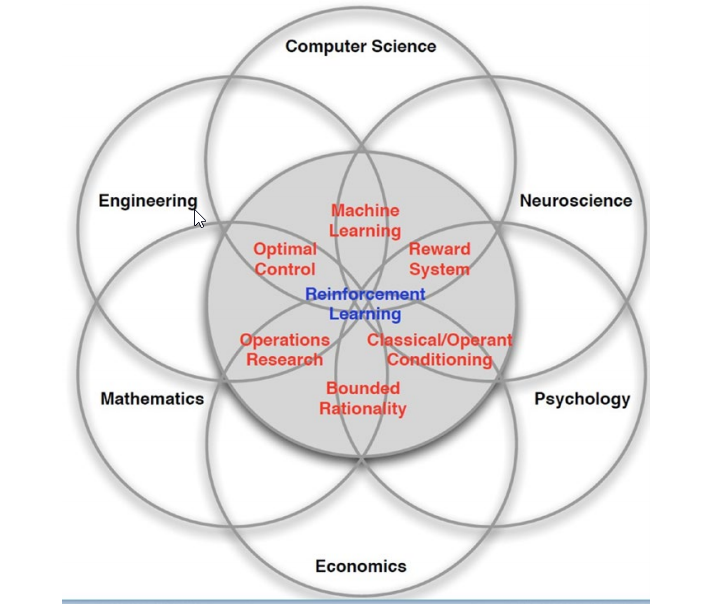
\includegraphics[scale=0.74]{Faces of Reinforcement Learning}
\caption{Venn diagram; }%from: \href{file:///H:/201906_fall/data/tmp/project2020-1/downloads/reinforcement_learning/2018_Book_ReinforcementLearning.pdf}{All the faces of Reinforcement Learning}
\end{center}
\end{figure}
\section{The Flow of Reinforcement Learning}
\begin{figure}[hbt!]
\begin{center}
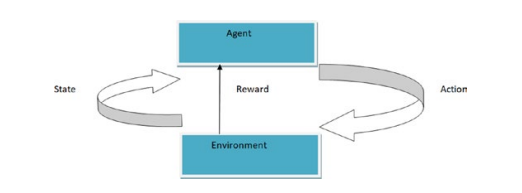
\includegraphics[scale=0.74]{The Flow of Reinforcement Learning}
\caption{RL structur}
\end{center}
\end{figure}
\begin{mini}\textbf{The key points of consideration:}\end{mini}\\
\begin{itemize}
\item The Reinforcement Learning cycle works in an interconnected. 
\end{itemize}

\begin{itemize}
\item The distinct communication happens with rewards in mind.
\end{itemize}
\begin{itemize}
\item There is distinct communication between the agent and the 
environment. 
 
\end{itemize}
\begin{itemize}
\item The object or robot moves from one state to another. 
 
\end{itemize}
\begin{itemize}
\item An action is taken to move from one state to another 
\end{itemize}

\begin{figure}[hbt!]
\begin{center}
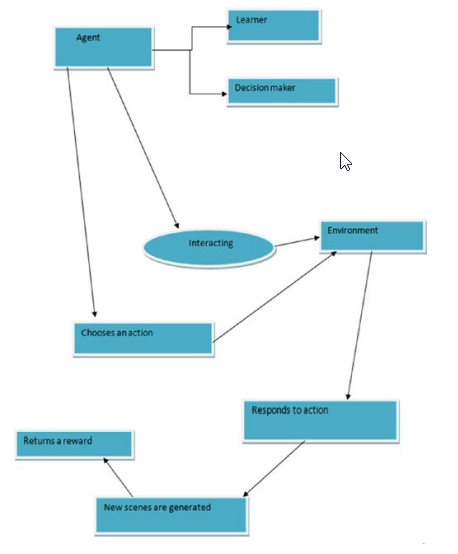
\includegraphics[scale=0.74]{The entire interaction process}
\caption{The entire interaction process; }%from: \href{file:///H:/201906_fall/data/tmp/project2020-1/downloads/reinforcement_learning/2018_Book_ReinforcementLearning.pdf}{All the faces of Reinforcement Learning}
\end{center}
\end{figure}
The agent is also a decision maker because it tries to take an action that will get it the 
maximum reward.\\
When the agent starts interacting with the environment, it can choose an action and 
respond accordingly.
From then on, new scenes are created. When the agent changes from one place to 
another in an environment, every change results in some kind of modification. These 
changes are depicted as scenes. The transition that happens in each step helps the agent 
solve the Reinforcement Learning problem more effectively\\
\begin{figure}[hbt!]
\begin{center}
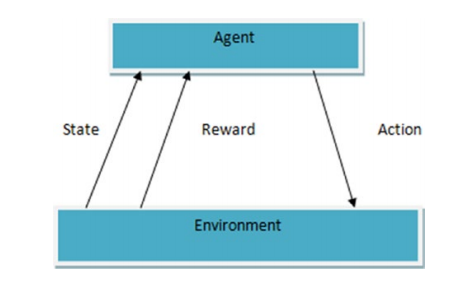
\includegraphics[scale=0.74]{ Scenario of state changes}
\caption{The entire interaction process; }%from: \href{file:///H:/201906_fall/data/tmp/project2020-1/downloads/reinforcement_learning/2018_Book_ReinforcementLearning.pdf}{All the faces of Reinforcement Learning}
\end{center}
\end{figure}
\section{Different Terms in Reinforcement Learning}
There are two constants that are important in this case—gamma (γ) and lambda (λ)\\[10pt]
Gamma is used in each state transition and is a constant value at each state change. 
Gamma allows you to give information about the type of reward you will be getting in 
every state. 
Gamma (γ) is called a discount 
factor and it determines what future reward types we get:\\
\begin{itemize}
\item A gamma value of 0 means the reward is associated with the 
current state only.
\end{itemize}

\begin{itemize}
\item A gamma value of 1 means that the reward is long-term.
\end{itemize}
Lambda is generally used when we are dealing with temporal difference problems. It is 
more involved with predictions in successive states.
Increasing values of lambda in each state shows that our algorithm is learning fast. 
The faster algorithm yields better results when using Reinforcement Learning techniques.
As you’ll learn later, temporal differences can be generalized to what we call 
TD(Lambda).\\

\section{Interactions with Reinforcement Learning}
\begin{figure}[hbt!]
\begin{center}
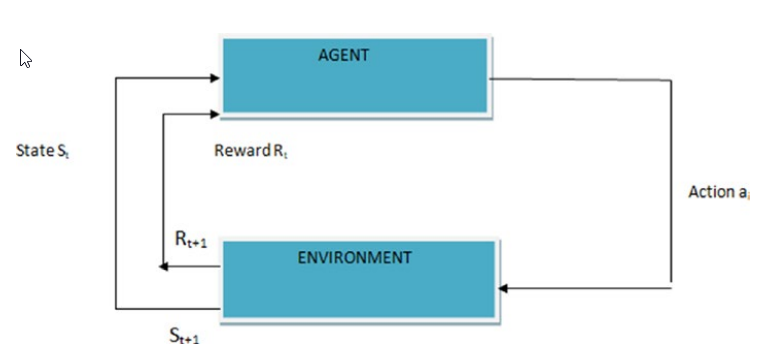
\includegraphics[scale=0.74]{ Reinforcement Learning interactions}
\caption{Reinforcement Learning interactions; }%from: \href{file:///H:/201906_fall/data/tmp/project2020-1/downloads/reinforcement_learning/2018_Book_ReinforcementLearning.pdf}{All the faces of Reinforcement Learning}
\end{center}
\end{figure}

The interactions between the agent and the environment occur with a reward. 
We need to take an action to move from one state to another.\\
Reinforcement Learning is a way of implementing how to map situations to actions 
so as to maximize and find a way to get the highest rewards.
The machine or robot is not told which actions to take, as with other forms of 
Machine Learning, but instead the machine must discover which actions yield the 
maximum reward by trying them.\\

\section{How Reward Works}
A reward is some motivator we receive when we transition from one state to another. It 
can be points, as in a video game. The more we train, the more accurate we become, and 
the greater our reward.\\

\section{Agents}
In terms of Reinforcement Learning, agents are the software programs that make
intelligent decisions. Agents should be able to perceive what is happening in the
environment. Here are the basic steps of the agents:\\
\begin{itemize}
\item When the agent can perceive the environment, it can make
better decisions.
\end{itemize}
\begin{itemize}
\item The decision the agents take results in an action.
\end{itemize}
\begin{itemize}
\item The action that the agents perform must be the best, the
optimal, one.
\end{itemize}

\begin{figure}[hbt!]
\begin{center}
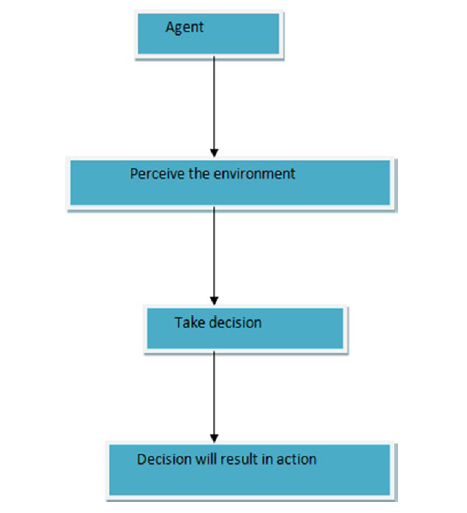
\includegraphics[scale=0.74]{agent}
\caption{agent}%from: \href{file:///H:/201906_fall/data/tmp/project2020-1/downloads/reinforcement_learning/2018_Book_ReinforcementLearning.pdf}{All the faces of Reinforcement Learning}
\end{center}
\end{figure}

\section{RL Environments}
The environments in the Reinforcement Learning space are comprised of certain factors
that determine the impact on the Reinforcement Learning agent. The agent must adapt
accordingly to the environment. These environments can be 2D worlds or grids or even a 3D world.\\
\begin{mini}\textbf{Here are some important features of environments:}\end{mini}\\
\begin{itemize}
\item Deterministic
\end{itemize}

\begin{itemize}
\item Observable
\end{itemize}
\begin{itemize}
\item Discrete or continuous
 
\end{itemize}
\begin{itemize}
\item Single or multiagent.
\end{itemize}
\end{document} 



